\titlespacing*{\section}
{0pt}{1ex plus 1ex minus .2ex}{-2.3ex plus .2ex}
\newcommand{\skipper}{\medskip\hrulefill\section{}}

\tikzset{state/.style={circle, draw, inner sep=4.3pt, opacity=1, fill=black, minimum size=0.2pt}}
\tikzset{statez/.style={draw, thick, inner sep=3.8pt, opacity=1, fill=black, minimum size=0.2pt}}
\tikzset{empty/.style={circle, draw, inner sep=4.3pt, opacity=0, fill=white, minimum size=0.2pt}}
    \tikzset{cross/.style={cross out, draw=black, minimum size=2*(#1-\pgflinewidth), inner sep=2pt, outer sep=2pt},
    %default radius will be 1pt. 
    cross/.default={1pt}}  
    \def \n {5} \def \radius {3cm} \def \raz {1.4cm}    \def \radiusz {4.5cm}
  
\newpage



    \centering
    
    \skipper 
    
    \begin{tikzpicture}[scale=0.65]

    \scriptsize
    
    
    \begin{scope}[xscale=-1]

    \foreach \s in {1,...,\n} { 
    \draw[dashed, >=latex] ({360/\n * (\s - 1)}:\radius)      arc ({360/\n * (\s - 1)}:{360/\n * (\s)}:\radius);   
    \draw[dotted, >=latex] ({360/\n * (\s - 2)+90}:\radius)      -- ({360/\n * (\s)+90}:\radius); 
    } 
    
    \node[state, fill=white] (1) at ({360/\n * (1 - 1)+90}:\radius) {};  
    \node[statez, fill=white] (1t) at ({360/\n * (1 - 1)+90}:\radius) {};  
    
    \node (01) at ({360/\n * (1 - 1)+90}:\radiusz) {};  
    \node[state, fill=white] (1a) at ({360/\n * (1 - 1)+90}:-\radius/2.618) {}; 
 
    
    \node[state, fill=blue] (2) at ({360/\n * (2 - 1)+90}:\radius){};   
    \node[statez, fill=blue] (2t) at ({360/\n * (2 - 1)+90}:\radius){};   
    \node (02) at ({360/\n * (2 - 1)+90}:\radiusz){};   
    \node[state, fill=blue] (2a) at ({360/\n * (2 - 1)+90}:-\radius/2.618) {}; 
    
    \node[state, fill=red] (3) at ({360/\n * (3 - 1)+90}:\radius) {};  
    \node[statez, fill=red] (3t) at ({360/\n * (3 - 1)+90}:\radius) {};  
    \node (03) at ({360/\n * (3 - 1)+90}:\radiusz) {};      
    \node[state, fill=red] (3a) at ({360/\n * (3 - 1)+90}:-\radius/2.618) {}; 
    
    \node[state, fill=yellow] (4) at ({360/\n * (4 - 1)+90}:\radius) {}; 
    \node[statez, fill=yellow] (4t) at ({360/\n * (4 - 1)+90}:\radius) {}; 
    \node (04) at ({360/\n * (4 - 1)+90}:\radiusz) {}; 
    \node[state, fill=yellow] (4a) at ({360/\n * (4 - 1)+90}:-\radius/2.618) {}; 
    
    \node[state, fill=green] (5) at ({360/\n * (5 - 1)+90}:\radius) {};   
    \node[statez, fill=green] (5t) at ({360/\n * (5 - 1)+90}:\radius) {};   
    \node (05) at ({360/\n * (5 - 1)+90}:\radiusz) {}; 
    \node[state, fill=green] (5a) at ({360/\n * (5 - 1)+90}:-\radius/2.618) {}; 
    
    
    \draw[>=triangle 45, line width=1.5pt, ->] (01) -- (1) ;
    \draw[>=triangle 45, line width=1.5pt, ->] (02) -- (2) ;
    \draw[>=triangle 45, line width=1.5pt, ->] (03) -- (3) ;
    \draw[>=triangle 45, line width=1.5pt, ->] (04) -- (4) ;
    \draw[>=triangle 45, line width=1.5pt, ->] (05) -- (5) ;    
    \end{scope}
    \end{tikzpicture}
    %\caption{Objective}
    
    Everyone has pieces of one \textbf{shape.}
    
    They start at the rim.
    
 

% \begin{multicols}{2}
% \raggedcolumns



 
  
\skipper % 2
    
    \begin{tikzpicture}[scale=0.65]

    \scriptsize
    \begin{scope}[xscale=-1]

    \foreach \s in {1,...,\n} { 
    \draw[dashed, >=latex] ({360/\n * (\s - 1)}:\radius)      arc ({360/\n * (\s - 1)}:{360/\n * (\s)}:\radius);   
    \draw[dotted, >=latex] ({360/\n * (\s - 2)+90}:\radius)      -- ({360/\n * (\s)+90}:\radius); 
    } 
    
    \node[state, fill=white] (1) at ({360/\n * (1 - 1)+90}:\radius) {};  
    \node[state, fill=white] (1a) at ({360/\n * (1 - 1)+90}:-\radius/2.618) {}; 
    \node[statez, fill=white] (1t) at ({360/\n * (1 - 1)+90}:-\radius/2.618) {}; 
    
    \node[state, fill=blue] (2) at ({360/\n * (2 - 1)+90}:\radius){};   
    \node[statez, fill=blue] (2t) at ({360/\n * (2 - 1)+90}:\radius){};       
    \node[state, fill=blue] (2a) at ({360/\n * (2 - 1)+90}:-\radius/2.618) {}; 
    
    \node[state, fill=red] (3) at ({360/\n * (3 - 1)+90}:\radius) {};  
    \node[statez, fill=red] (3t) at ({360/\n * (3 - 1)+90}:\radius) {};  
    \node[state, fill=red] (3a) at ({360/\n * (3 - 1)+90}:-\radius/2.618) {}; 
    
    \node[state, fill=yellow] (4) at ({360/\n * (4 - 1)+90}:\radius) {}; 
    \node[statez, fill=yellow] (4t) at ({360/\n * (4 - 1)+90}:\radius) {};     
    \node[state, fill=yellow] (4a) at ({360/\n * (4 - 1)+90}:-\radius/2.618) {}; 
    
    \node[state, fill=green] (5) at ({360/\n * (5 - 1)+90}:\radius) {};   
    \node[statez, fill=green] (5t) at ({360/\n * (5 - 1)+90}:\radius) {};       
    \node[state, fill=green] (5a) at ({360/\n * (5 - 1)+90}:-\radius/2.618) {}; 
    
    
    \draw[>=triangle 45, dashed, line width=1.5pt, ->] (1) -- (1a) ;
    \end{scope}
    \end{tikzpicture}
    %\caption{Objective}
    
   
     
    
    All white pieces travel to white, blue to blue etc.
    
    \textbf{Three out wins.}

% \begin{multicols}{2}
% \raggedcolumns



   \skipper

      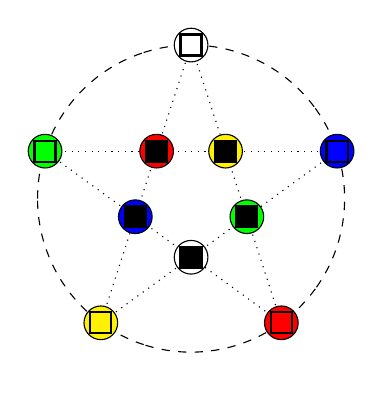
\begin{tikzpicture}[scale=0.65]

    \scriptsize
    \begin{scope}[xscale=-1]

    \foreach \s in {1,...,\n} { 
    \draw[dashed, >=latex] ({360/\n * (\s - 1)}:\radius)      arc ({360/\n * (\s - 1)}:{360/\n * (\s)}:\radius);   
    \draw[dotted, >=latex] ({360/\n * (\s - 2)+90}:\radius)      -- ({360/\n * (\s)+90}:\radius); 
    } 
    
    \node[state, fill=white] (1) at ({360/\n * (1 - 1)+90}:\radius) {};  
    \node[statez, fill=white] (1t) at ({360/\n * (1 - 1)+90}:\radius) {};  
    \node[state, fill=white] (1a) at ({360/\n * (1 - 1)+90}:-\radius/2.618) {}; 
    \node[statez, fill=black] (1a) at ({360/\n * (1 - 1)+90}:-\radius/2.618) {}; 
    
    \node[state, fill=blue] (2) at ({360/\n * (2 - 1)+90}:\radius){};   
    \node[statez, fill=blue] (2t) at ({360/\n * (2 - 1)+90}:\radius){};   
    \node[state, fill=blue] (2a) at ({360/\n * (2 - 1)+90}:-\radius/2.618) {}; 
    \node[statez, fill=black] (2a) at ({360/\n * (2 - 1)+90}:-\radius/2.618) {}; 
    
    \node[state, fill=red] (3) at ({360/\n * (3 - 1)+90}:\radius) {};  
    \node[statez, fill=red] (3t) at ({360/\n * (3 - 1)+90}:\radius) {};      
    \node[state, fill=red] (3a) at ({360/\n * (3 - 1)+90}:-\radius/2.618) {}; 
    \node[statez, fill=black] (3a) at ({360/\n * (3 - 1)+90}:-\radius/2.618) {}; 
    
    \node[state, fill=yellow] (4) at ({360/\n * (4 - 1)+90}:\radius) {}; 
    \node[statez, fill=yellow] (4t) at ({360/\n * (4 - 1)+90}:\radius) {};     
    \node[state, fill=yellow] (4a) at ({360/\n * (4 - 1)+90}:-\radius/2.618) {}; 
    \node[statez, fill=black] (4a) at ({360/\n * (4 - 1)+90}:-\radius/2.618) {}; 
    
    \node[state, fill=green] (5) at ({360/\n * (5 - 1)+90}:\radius) {};   
    \node[statez, fill=green] (5t) at ({360/\n * (5 - 1)+90}:\radius) {};       
    \node[state, fill=green] (5a) at ({360/\n * (5 - 1)+90}:-\radius/2.618) {}; 
    \node[statez, fill=black] (5a) at ({360/\n * (5 - 1)+90}:-\radius/2.618) {};     
    
    \end{scope}
    \end{tikzpicture}
    %\caption{Objective}
    
   
    Put black blocks on the crossings.
    
    They are neutral.

  
\skipper 


% \begin{multicols}{2}
% \raggedcolumns



 

    \begin{tikzpicture}[scale=0.65]
    \scriptsize
    \begin{scope}[xscale=-1]

    \foreach \s in {1,...,\n} { 
    \draw[dashed, >=latex] ({360/\n * (\s - 1)}:\radius)      arc ({360/\n * (\s - 1)}:{360/\n * (\s)}:\radius);   
    \draw[dotted, >=latex] ({360/\n * (\s - 2)+90}:\radius)      -- ({360/\n * (\s)+90}:\radius); 
    } 
    %\draw[dashed] ({360/\n * (1 - 1)+95}:\radius)      arc ({360/\n * (1 - 1)+95}:{360/\n * (1)+85}:\radius)  node[midway, rotate=-18] {$\times$};
    \draw[>=triangle 45, line width=1.5pt, ->] ({360/\n * (1-1)+95}:\radius)  arc ({360/\n * (1-1)+95}:{360/\n * (2-1)+80}:\radius) node[midway,left]{};
    
    \draw[>=triangle 45, line width=1.5pt, ->] ({360/\n * (1-1)+95}:\radius)  arc ({360/\n * (1-1)+95}:{360/\n * (-1)+100}:\radius) node[midway,left]{};
    
    \draw[>=triangle 45, line width=1.5pt, shorten >=1.5ex, ->] (1) -- (4a);
    
    \draw[>=triangle 45, line width=1.5pt, shorten >=1.5ex, ->] (1) -- (3a);
    
    
    \node[state, fill=white] (1) at ({360/\n * (1 - 1)+90}:\radius) {};  
    \node[statez, fill=white] (1t) at ({360/\n * (1 - 1)+90}:\radius) {};      
    \node[state, fill=white] (1a) at ({360/\n * (1 - 1)+90}:-\radius/2.618) {}; 
    
    \node[state, fill=blue] (2) at ({360/\n * (2 - 1)+90}:\radius){};   
    \node[state, fill=blue] (2a) at ({360/\n * (2 - 1)+90}:-\radius/2.618) {}; 
    
    \node[state, fill=red] (3) at ({360/\n * (3 - 1)+90}:\radius) {};  
    \node[state, fill=red] (3a) at ({360/\n * (3 - 1)+90}:-\radius/2.618) {}; 
    
    \node[state, fill=yellow] (4) at ({360/\n * (4 - 1)+90}:\radius) {}; 
    \node[state, fill=yellow] (4a) at ({360/\n * (4 - 1)+90}:-\radius/2.618) {}; 
    
    \node[state, fill=green] (5) at ({360/\n * (5 - 1)+90}:\radius) {};   
    \node[state, fill=green] (5a) at ({360/\n * (5 - 1)+90}:-\radius/2.618) {}; 
    
    \end{scope}
    \end{tikzpicture}
    %\caption{Simple move on ring}
    
    You can move \textbf{in any direction,} on the ring and on the star.
    
 \skipper

    %%%% EXAMPLE MOVES
    \centering
    \begin{tikzpicture}[scale=0.65]
    \scriptsize
    \begin{scope}[xscale=-1]

    \foreach \s in {1,...,\n} { 
    \draw[dashed, >=latex] ({360/\n * (\s - 1)}:\radius)      arc ({360/\n * (\s - 1)}:{360/\n * (\s)}:\radius);   
    \draw[dotted, >=latex] ({360/\n * (\s - 2)+90}:\radius)      -- ({360/\n * (\s)+90}:\radius); 
    } 
    
    \node[state, fill=white] (1) at ({360/\n * (1 - 1)+90}:\radius) {};  
    \node[statez, fill=white] (1t) at ({360/\n * (1 - 1)+90}:\radius) {};  
    \node[state, fill=white] (1a) at ({360/\n * (1 - 1)+90}:-\radius/2.618) {};
    \node[statez, fill=black] (1z) at ({360/\n * (1 - 1)+90}:-\radius/2.618) {}; 
    
    \node[state, fill=blue] (2) at ({360/\n * (2 - 1)+90}:\radius){};   
    \node[statez, fill=blue] (2t) at ({360/\n * (2 - 1)+90}:\radius){};   
    \node[state, fill=blue] (2a) at ({360/\n * (2 - 1)+90}:-\radius/2.618) {};
    \node[statez, fill=black] (2z) at ({360/\n * (2 - 1)+90}:-\radius/2.618) {}; 
    
    \node[state, fill=red] (3) at ({360/\n * (3 - 1)+90}:\radius) {};  
    \node[statez, fill=red] (3t) at ({360/\n * (3 - 1)+90}:\radius) {};  
    \node[state, fill=red] (3a) at ({360/\n * (3 - 1)+90}:-\radius/2.618) {}; 
    \node[statez, fill=black] (3z) at ({360/\n * (3 - 1)+90}:-\radius/2.618) {};     
    
    \node[state, fill=yellow] (4) at ({360/\n * (4 - 1)+90}:\radius) {}; 
    \node[statez, fill=yellow] (4t) at ({360/\n * (4 - 1)+90}:\radius) {};     
    \node[state, fill=yellow] (4a) at ({360/\n * (4 - 1)+90}:-\radius/2.618) {}; 
    \node[statez, fill=black] (4z) at ({360/\n * (4 - 1)+90}:-\radius/2.618) {}; 
    
    \node[state, fill=green] (5) at ({360/\n * (5 - 1)+90}:\radius) {};   
    \node[statez, fill=green] (5t) at ({360/\n * (5 - 1)+90}:\radius) {};       
    \node[state, fill=green] (5a) at ({360/\n * (5 - 1)+90}:-\radius/2.618) {}; 
    \node[statez, fill=black] (5z) at ({360/\n * (5 - 1)+90}:-\radius/2.618) {};     
    
    \draw[>=triangle 45, line width=1.5pt, shorten >=1.5ex, ->] (1) -- (4a);
    \end{scope}
    \end{tikzpicture}
    %\caption{Simple move}
    
    You can move \textbf{as far as you want.}
    
    But:\textbf{ you cannot jump!}
     
    
   
    \skipper
    \begin{tikzpicture}[scale=0.65]
    \scriptsize
    \begin{scope}[xscale=-1]

    \foreach \s in {1,...,\n} { 
    \draw[dashed, >=latex] ({360/\n * (\s - 1)}:\radius)      arc ({360/\n * (\s - 1)}:{360/\n * (\s)}:\radius);   
    \draw[dotted, >=latex] ({360/\n * (\s - 2)+90}:\radius)      -- ({360/\n * (\s)+90}:\radius); 
    } 
    
    \node[state, fill=white] (1) at ({360/\n * (1 - 1)+90}:\radius) {};  
    \node[state, fill=white] (1a) at ({360/\n * (1 - 1)+90}:-\radius/2.618) {}; 
    \node[statez, fill=black] (1z) at ({360/\n * (1 - 1)+90}:-\radius/2.618) {}; 
    
    \node[state, fill=blue] (2) at ({360/\n * (2 - 1)+90}:\radius){};   
    \node[state, fill=blue] (2a) at ({360/\n * (2 - 1)+90}:-\radius/2.618) {}; 
    \node[statez, fill=black] (2z) at ({360/\n * (2 - 1)+90}:-\radius/2.618) {};
    
    \node[state, fill=red] (3) at ({360/\n * (3 - 1)+90}:\radius) {};  
    \node[state, fill=red] (3a) at ({360/\n * (3 - 1)+90}:-\radius/2.618) {}; 
    \node[statez, fill=black] (3a) at ({360/\n * (3 - 1)+90}:-\radius/2.618) {};     
    
    \node[state, fill=yellow] (4) at ({360/\n * (4 - 1)+90}:\radius) {}; 
    \node[state, fill=yellow] (4a) at ({360/\n * (4 - 1)+90}:-\radius/2.618) {}; 
    \node[statez, fill=white] (4z) at ({360/\n * (4 - 1)+90}:-\radius/2.618) {}; 
        
    \node[state, fill=green] (5) at ({360/\n * (5 - 1)+90}:\radius) {};   
    \node[state, fill=green] (5a) at ({360/\n * (5 - 1)+90}:-\radius/2.618) {}; 
    \node[statez, fill=black] (5z) at ({360/\n * (5 - 1)+90}:-\radius/2.618) {};     
    
    \draw[>=triangle 45, line width=1.5pt, ->] (1) -- (4a) node[midway,right]{$hit$};
    
    \draw[dashed, >=triangle 45, line width=1.5pt, ->] (4a) -- (-2.8,-1) node[midway,right]{$replace$};
    
    \end{scope}
    \end{tikzpicture}
    %\caption{Replace a block}
    
    You can \textbf{hit a black block.} 
    
    You then \textbf{replace} it on another empty space.
    
    


  
    \skipper
    \begin{tikzpicture}[scale=0.65]
    \scriptsize
    \begin{scope}[xscale=-1]

    \foreach \s in {1,...,\n} { 
    \draw[dashed, >=latex] ({360/\n * (\s - 1)}:\radius)      arc ({360/\n * (\s - 1)}:{360/\n * (\s)}:\radius);   
    \draw[dotted, >=latex] ({360/\n * (\s - 2)+90}:\radius)      -- ({360/\n * (\s)+90}:\radius); 
    } 
    %\draw[dashed] ({360/\n * (1 - 1)+95}:\radius)      arc ({360/\n * (1 - 1)+95}:{360/\n * (1)+85}:\radius)  node[midway, rotate=-18] {$\times$};
    \draw[>=triangle 45, style=double, line width=0.5pt, <->] ({360/\n * (1-1)+95}:\radius)  arc ({360/\n * (1-1)+95}:{360/\n * (2-1)+85}:\radius) node[midway,right]{$swap$};
    
    %\draw[line width=1.5pt, -] ({360/\n * (1)+90}:\radius)      arc ({360/\n * (1)+90}:{360/\n * (2)+90}:\radius) node[midway,below]{};
    
    \node[state, fill=white] (1) at ({360/\n * (1 - 1)+90}:\radius) {};  
    \node[statez, fill=blue] (1t) at ({360/\n * (1 - 1)+90}:\radius) {};      
    \node[state, fill=white] (1a) at ({360/\n * (1 - 1)+90}:-\radius/2.618) {}; 
    
    \node[state, fill=blue] (2) at ({360/\n * (2 - 1)+90}:\radius){};   
    \node[statez, fill=white] (2t) at ({360/\n * (2 - 1)+90}:\radius){};       
    \node[state, fill=blue] (2a) at ({360/\n * (2 - 1)+90}:-\radius/2.618) {}; 
    
    \node[state, fill=red] (3) at ({360/\n * (3 - 1)+90}:\radius) {};  
    \node[state, fill=red] (3a) at ({360/\n * (3 - 1)+90}:-\radius/2.618) {}; 
    
    \node[state, fill=yellow] (4) at ({360/\n * (4 - 1)+90}:\radius) {}; 
    \node[state, fill=yellow] (4a) at ({360/\n * (4 - 1)+90}:-\radius/2.618) {}; 
    
    \node[state, fill=green] (5) at ({360/\n * (5 - 1)+90}:\radius) {};   
    \node[state, fill=green] (5a) at ({360/\n * (5 - 1)+90}:-\radius/2.618) {}; 
    
    \end{scope}
    \end{tikzpicture}
    %\caption{Swap two pieces}
    
    You can \textbf{swap} two neighbouring pieces \\ (at least one of which must be yours). 
    
    Of course the way must be free!
    
            \skipper
    
    
    \begin{tikzpicture}[scale=0.65]
    \scriptsize
    \begin{scope}[xscale=-1]

    \foreach \s in {1,...,\n} { 
    \draw[dashed, >=latex] ({360/\n * (\s - 1)}:\radius)      arc ({360/\n * (\s - 1)}:{360/\n * (\s)}:\radius);   
    \draw[dotted, >=latex] ({360/\n * (\s - 2)+90}:\radius)      -- ({360/\n * (\s)+90}:\radius); 
    } 
    
    \node[state, fill=white] (1) at ({360/\n * (1 - 1)+90}:\radius) {};  
    \node[state, fill=white] (1a) at ({360/\n * (1 - 1)+90}:-\radius/2.618) {}; 
    \node[statez, fill=white] (1t) at ({360/\n * (1 - 1)+90}:-\radius/2.618) {};     
    
    \node[state, fill=blue] (2) at ({360/\n * (2 - 1)+90}:\radius){};   
    \node[state, fill=blue] (2a) at ({360/\n * (2 - 1)+90}:-\radius/2.618) {}; 
    
    \node[state, fill=red] (3) at ({360/\n * (3 - 1)+90}:\radius) {};  
    \node[state, fill=red] (3a) at ({360/\n * (3 - 1)+90}:-\radius/2.618) {}; 
    
    \node[state, fill=yellow] (4) at ({360/\n * (4 - 1)+90}:\radius) {}; 
    \node[state, fill=yellow] (4a) at ({360/\n * (4 - 1)+90}:-\radius/2.618) {}; 
    
    \node[state, fill=green] (5) at ({360/\n * (5 - 1)+90}:\radius) {};   
    \node[state, fill=green] (5a) at ({360/\n * (5 - 1)+90}:-\radius/2.618) {}; 
    
    
    \draw[dashed, >=triangle 45, line width=1.5pt, ->] (1) -- (1a);
    
    \draw[>=triangle 45, line width=1.5pt, ->] (1a) -- (1,-1) node[left]{out};
    
    \draw[>=triangle 45, line width=1.5pt, ->] (-0.4,0) -- (-2.4,1.7) node[right]{grey};
    
    
    \end{scope}
    \end{tikzpicture}
    %\caption{Move out, set a new gray block}
    
    When you \textbf{reach a goal,} your piece moves \textbf{out. }
    
    For this you \textbf{place a grey block} anywhere.
    
    Grey blocks are \textbf{one-time blocks.}
    
    
    

    %%%% TURN CORNERS
  
    \skipper
    \begin{tikzpicture}[scale=0.65]
    \scriptsize
    \begin{scope}[xscale=-1]

    \foreach \s in {1,...,\n} { 
    \draw[dashed, >=latex] ({360/\n * (\s - 1)}:\radius)      arc ({360/\n * (\s - 1)}:{360/\n * (\s)}:\radius);   
    \draw[dotted, >=latex] ({360/\n * (\s - 2)+90}:\radius)      -- ({360/\n * (\s)+90}:\radius); 
    } 
    
    \node[state, fill=white] (1) at ({360/\n * (1 - 1)+90}:\radius) {};  
    \node[state, fill=white] (1a) at ({360/\n * (1 - 1)+90}:-\radius/2.618) {}; 
    \node[statez, fill=white] (1t) at ({360/\n * (1 - 1)+90}:-\radius/2.618) {}; 
    
    \node[state, fill=blue] (2) at ({360/\n * (2 - 1)+90}:\radius){};   
    \node[statez, fill=black] (2t) at ({360/\n * (2 - 1)+90}:\radius){};       
    \node[state, fill=blue] (2a) at ({360/\n * (2 - 1)+90}:-\radius/2.618) {}; 
    \node[statez, fill=black] (2z) at ({360/\n * (2 - 1)+90}:-\radius/2.618) {}; 
    
    \node[state, fill=red] (3) at ({360/\n * (3 - 1)+90}:\radius) {};  
    \node[statez, fill=black] (3t) at ({360/\n * (3 - 1)+90}:\radius) {};      
    \node[state, fill=red] (3a) at ({360/\n * (3 - 1)+90}:-\radius/2.618) {}; 
    \node[statez, fill=black] (3z) at ({360/\n * (3 - 1)+90}:-\radius/2.618) {};     
    
    \node[state, fill=yellow] (4) at ({360/\n * (4 - 1)+90}:\radius) {}; 
    \node[statez, fill=black] (4z) at ({360/\n * (4 - 1)+90}:\radius) {};     
    \node[state, fill=yellow] (4a) at ({360/\n * (4 - 1)+90}:-\radius/2.618) {}; 
    
    \node[state, fill=green] (5) at ({360/\n * (5 - 1)+90}:\radius) {};   
    \node[statez, fill=black] (5z) at ({360/\n * (5 - 1)+90}:\radius) {};       
    \node[state, fill=green] (5a) at ({360/\n * (5 - 1)+90}:-\radius/2.618) {}; 
    
    
    \draw[>=triangle 45, line width=1.5pt, -] (1) -- (4a) node[midway,right]{};
    \draw[>=triangle 45, line width=1.5pt, -] (4a) -- (5a) node[midway,right]{$turn$};
    \draw[>=triangle 45, line width=1.5pt, ->] (5a) -- (1a) node[midway,left]{};
    
    \end{scope}
    \end{tikzpicture}
    
    %\caption{Turn corners on free paths}
    
    \textbf{Turn} at free corners without stopping. 

    Ways can be long!
    
    

  

    \skipper

\raggedright

\vspace{5ex}

Edge cases:

    \begin{enumerate}
        \item When moving to a corner with multiple pieces, swap with one of them.
        \item You can't try the same twice.
        \item When you get to set both a grey and a black block say `Abracadabra'.
        \item You cannot move out when it is not your turn.
        \item When it is your turn and one of your pieces was brought to its goal by someone else, then you must move that piece out, gaining a grey block. You do not have another move.
        \item When you need more grey blocks than there are re-position one.
    \end{enumerate}

\hrulefill

%\skipper

%\vspace{5ex}


%Please visit \website ! 


%\end{multicols}